

\tikzset{every picture/.style={line width=0.75pt}} %set default line width to 0.75pt        

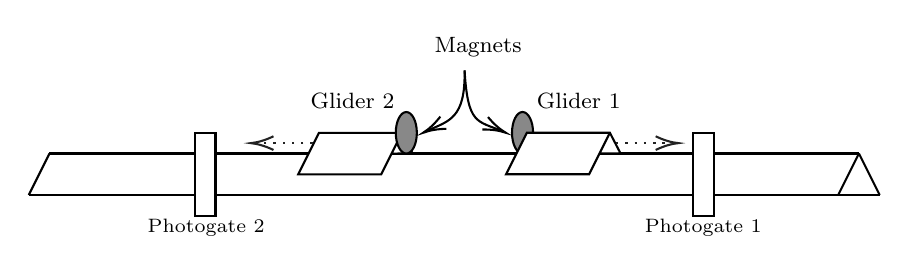
\begin{tikzpicture}[x=0.75pt,y=0.75pt,yscale=-1,xscale=1]
%uncomment if require: \path (0,300); %set diagram left start at 0, and has height of 300

%Straight Lines [id:da5572434639926174] 
\draw    (110,140) -- (520,140) ;


%Straight Lines [id:da02244511382700587] 
\draw    (110,140) -- (120,120) ;


%Straight Lines [id:da5497476983892675] 
\draw    (120,120) -- (510,120) ;


%Straight Lines [id:da57322939128216] 
\draw    (510,120) -- (520,140) ;


%Straight Lines [id:da2970462263374636] 
\draw    (510,120) -- (500,140) ;


%Shape: Rectangle [id:dp04813805212125999] 
\draw  [fill={rgb, 255:red, 255; green, 255; blue, 255 }  ,fill opacity=1 ] (190,110) -- (200,110) -- (200,150) -- (190,150) -- cycle ;
%Shape: Rectangle [id:dp8954323751602662] 
\draw  [fill={rgb, 255:red, 255; green, 255; blue, 255 }  ,fill opacity=1 ] (430,110) -- (440,110) -- (440,150) -- (430,150) -- cycle ;
%Shape: Polygon [id:ds6910058608548333] 
\draw  [fill={rgb, 255:red, 255; green, 255; blue, 255 }  ,fill opacity=1 ] (249.85,110.02) -- (289.85,110.02) -- (295,120) -- (284.85,120.02) -- (289.85,110.02) -- (279.85,130.02) -- (239.85,130.02) -- cycle ;
%Shape: Ellipse [id:dp9683169570061398] 
\draw  [fill={rgb, 255:red, 136; green, 136; blue, 136 }  ,fill opacity=1 ] (286.85,110.02) .. controls (286.85,104.5) and (289.12,100.02) .. (291.93,100.02) .. controls (294.73,100.02) and (297,104.5) .. (297,110.02) .. controls (297,115.54) and (294.73,120.02) .. (291.93,120.02) .. controls (289.12,120.02) and (286.85,115.54) .. (286.85,110.02) -- cycle ;
%Shape: Ellipse [id:dp16081275394461825] 
\draw  [fill={rgb, 255:red, 136; green, 136; blue, 136 }  ,fill opacity=1 ] (342.85,110) .. controls (342.85,104.48) and (345.12,100) .. (347.93,100) .. controls (350.73,100) and (353,104.48) .. (353,110) .. controls (353,115.52) and (350.73,120) .. (347.93,120) .. controls (345.12,120) and (342.85,115.52) .. (342.85,110) -- cycle ;
%Curve Lines [id:da16877543821086127] 
\draw    (320,80) .. controls (320.42,103.4) and (312.5,104.21) .. (301.72,109.19) ;
\draw [shift={(300,110.02)}, rotate = 333.58000000000004] [color={rgb, 255:red, 0; green, 0; blue, 0 }  ][line width=0.75]    (10.93,-3.29) .. controls (6.95,-1.4) and (3.31,-0.3) .. (0,0) .. controls (3.31,0.3) and (6.95,1.4) .. (10.93,3.29)   ;

%Curve Lines [id:da546070735716643] 
\draw    (320,80) .. controls (321.57,106.2) and (326.01,104.1) .. (338.09,109.22) ;
\draw [shift={(339.85,110)}, rotate = 204.68] [color={rgb, 255:red, 0; green, 0; blue, 0 }  ][line width=0.75]    (10.93,-3.29) .. controls (6.95,-1.4) and (3.31,-0.3) .. (0,0) .. controls (3.31,0.3) and (6.95,1.4) .. (10.93,3.29)   ;

%Shape: Polygon [id:ds012853840364027702] 
\draw  [fill={rgb, 255:red, 255; green, 255; blue, 255 }  ,fill opacity=1 ] (350,110) -- (390,110) -- (395.15,119.98) -- (385,120) -- (390,110) -- (380,130) -- (340,130) -- cycle ;
%Straight Lines [id:da4347205803244891] 
\draw [color={rgb, 255:red, 34; green, 34; blue, 34 }  ,draw opacity=1 ] [dash pattern={on 0.84pt off 2.51pt}]  (246.85,115) -- (219,115) ;
\draw [shift={(217,115)}, rotate = 360] [color={rgb, 255:red, 34; green, 34; blue, 34 }  ,draw opacity=1 ][line width=0.75]    (10.93,-3.29) .. controls (6.95,-1.4) and (3.31,-0.3) .. (0,0) .. controls (3.31,0.3) and (6.95,1.4) .. (10.93,3.29)   ;

%Straight Lines [id:da1823174319264671] 
\draw [color={rgb, 255:red, 34; green, 34; blue, 34 }  ,draw opacity=1 ] [dash pattern={on 0.84pt off 2.51pt}]  (393,115) -- (421,115) ;
\draw [shift={(423,115)}, rotate = 180] [color={rgb, 255:red, 34; green, 34; blue, 34 }  ,draw opacity=1 ][line width=0.75]    (10.93,-3.29) .. controls (6.95,-1.4) and (3.31,-0.3) .. (0,0) .. controls (3.31,0.3) and (6.95,1.4) .. (10.93,3.29)   ;


% Text Node
\draw (435,155.5) node  [font=\footnotesize] [align=left] {{\scriptsize Photogate 1}};
% Text Node
\draw (195.5,155.5) node  [font=\footnotesize] [align=left] {{\scriptsize Photogate 2}};
% Text Node
\draw (266,94.5) node  [font=\scriptsize] [align=left] {{\footnotesize Glider 2}};
% Text Node
\draw (375,94.5) node  [font=\scriptsize] [align=left] {{\footnotesize Glider 1}};
% Text Node
\draw (326.5,68.5) node  [font=\footnotesize] [align=left] {Magnets};


\end{tikzpicture}
